\iffalse
\documentclass[journal,12pt,twocolumn]{IEEEtran}
%
\usepackage{setspace}
\usepackage{gensymb}
%\doublespacing
\singlespacing

%\usepackage{graphicx}
%\usepackage{amssymb}
%\usepackage{relsize}
\usepackage[cmex10]{amsmath}
\usepackage{siunitx}
%\usepackage{amsthm}
%\interdisplaylinepenalty=2500
%\savesymbol{iint}
%\usepackage{txfonts}
%\restoresymbol{TXF}{iint}
%\usepackage{wasysym}
\usepackage{amsthm}
%\usepackage{iithtlc}
\usepackage{mathrsfs}
\usepackage{txfonts}
\usepackage{stfloats}
\usepackage{steinmetz}
\usepackage{supertabular}
%\usepackage{bm}
\usepackage{cite}
\usepackage{cases}
\usepackage{subfig}
%\usepackage{xtab}
\usepackage{longtable}
\usepackage{multirow}
%\usepackage{algorithm}
%\usepackage{algpseudocode}
\usepackage{enumitem}
\usepackage{mathtools}
\usepackage{tikz}
\usepackage{circuitikz}
\usepackage{verbatim}
\usepackage{tfrupee}
\usepackage[breaklinks=true]{hyperref}
%\usepackage{stmaryrd}
\usepackage{tkz-euclide} % loads  TikZ and tkz-base
%\usetkzobj{all}
\usetikzlibrary{calc,math}
\usetikzlibrary{fadings}
\usepackage{listings}
    \usepackage{color}                                            %%
    \usepackage{array}                                            %%
    \usepackage{longtable}                                        %%
    \usepackage{calc}                                             %%
    \usepackage{multirow}                                         %%
    \usepackage{hhline}                                           %%
    \usepackage{ifthen}                                           %%
  %optionally (for landscape tables embedded in another document): %%
    \usepackage{lscape}     
\usepackage{multicol}
\usepackage{chngcntr}
\usepackage{blkarray}
\usepackage{karnaugh-map}
\usepackage{fontspec}
\usepackage[intoc]{nomencl}
\makenomenclature

%\usetikzlibrary{arrows, shapes.gates.logic.US, calc}
\usetikzlibrary{arrows,shapes.gates.logic.US,shapes.gates.logic.IEC,calc}
\setmainfont{Sanskrit_2003.ttf}
%\setmainfont{Nakula.ttf}
%\setmainfont{Lohit-Devanagari.ttf}


%\usepackage{enumerate}

%\usepackage{wasysym}
%\newcounter{MYtempeqncnt}
\DeclareMathOperator*{\Res}{Res}
%\renewcommand{\baselinestretch}{2}
\renewcommand\thesection{\arabic{section}}
\renewcommand\thesubsection{\thesection.\arabic{subsection}}
\renewcommand\thesubsubsection{\thesubsection.\arabic{subsubsection}}

\renewcommand\thesectiondis{\arabic{section}}
\renewcommand\thesubsectiondis{\thesectiondis.\arabic{subsection}}
\renewcommand\thesubsubsectiondis{\thesubsectiondis.\arabic{subsubsection}}

% correct bad hyphenation here
\hyphenation{op-tical net-works semi-conduc-tor}
\def\inputGnumericTable{}                                 %%


\lstset{
%language=shell,
%language = Prolog,
frame=single, 
breaklines=true,
%showstringspaces=false,
columns=fullflexible
literate = {-}{-}1
}
%\lstset{
%language=tex,
%frame=single, 
%breaklines=true
%}

\begin{document}
%


\newtheorem{theorem}{Theorem}[section]
\newtheorem{problem}{Problem}
\newtheorem{proposition}{Proposition}[section]
\newtheorem{lemma}{Lemma}[section]
\newtheorem{corollary}[theorem]{Corollary}
\newtheorem{example}{Example}[section]
\newtheorem{definition}[problem]{Definition}
%\newtheorem{thm}{Theorem}[section] 
%\newtheorem{defn}[thm]{Definition}
%\newtheorem{algorithm}{Algorithm}[section]
%\newtheorem{cor}{Corollary}
\newcommand{\BEQA}{\begin{eqnarray}}
\newcommand{\EEQA}{\end{eqnarray}}
\newcommand{\define}{\stackrel{\triangle}{=}}

\bibliographystyle{IEEEtran}
%\bibliographystyle{ieeetr}


\providecommand{\mbf}{\mathbf}
\providecommand{\pr}[1]{\ensuremath{\Pr\left(#1\right)}}
\providecommand{\qfunc}[1]{\ensuremath{Q\left(#1\right)}}
\providecommand{\sbrak}[1]{\ensuremath{{}\left[#1\right]}}
\providecommand{\lsbrak}[1]{\ensuremath{{}\left[#1\right.}}
\providecommand{\rsbrak}[1]{\ensuremath{{}\left.#1\right]}}
\providecommand{\brak}[1]{\ensuremath{\left(#1\right)}}
\providecommand{\lbrak}[1]{\ensuremath{\left(#1\right.}}
\providecommand{\rbrak}[1]{\ensuremath{\left.#1\right)}}
\providecommand{\cbrak}[1]{\ensuremath{\left\{#1\right\}}}
\providecommand{\lcbrak}[1]{\ensuremath{\left\{#1\right.}}
\providecommand{\rcbrak}[1]{\ensuremath{\left.#1\right\}}}
\providecommand{\ceil}[1]{\left \lceil #1 \right \rceil }
\theoremstyle{remark}
\newtheorem{rem}{Remark}
\newcommand{\sgn}{\mathop{\mathrm{sgn}}}
\providecommand{\abs}[1]{\left\vert#1\right\vert}
\providecommand{\res}[1]{\Res\displaylimits_{#1}} 
\providecommand{\norm}[1]{\left\lVert#1\right\rVert}
%\providecommand{\norm}[1]{\lVert#1\rVert}
\providecommand{\mtx}[1]{\mathbf{#1}}
\providecommand{\mean}[1]{E\left[ #1 \right]}
\providecommand{\fourier}{\overset{\mathcal{F}}{ \rightleftharpoons}}
%\providecommand{\hilbert}{\overset{\mathcal{H}}{ \rightleftharpoons}}
\providecommand{\system}{\overset{\mathcal{H}}{ \longleftrightarrow}}
	%\newcommand{\solution}[2]{\textbf{Solution:}{#1}}
\newcommand{\solution}{\noindent \textbf{Solution: }}
\newcommand{\cosec}{\,\text{cosec}\,}
\providecommand{\dec}[2]{\ensuremath{\overset{#1}{\underset{#2}{\gtrless}}}}
\newcommand{\myvec}[1]{\ensuremath{\begin{pmatrix}#1\end{pmatrix}}}
\newcommand{\mydet}[1]{\ensuremath{\begin{vmatrix}#1\end{vmatrix}}}
%\numberwithin{equation}{section}
\numberwithin{equation}{subsection}
%\numberwithin{problem}{section}
%\numberwithin{definition}{section}
\makeatletter
\@addtoreset{figure}{problem}
\makeatother

\let\StandardTheFigure\thefigure
\let\vec\mathbf
%\renewcommand{\thefigure}{\theproblem.\arabic{figure}}
%\renewcommand{\thefigure}{\theproblem}
\renewcommand{\thefigure}{\thesection}
%\setlist[enumerate,1]{before=\renewcommand\theequation{\theenumi.\arabic{equation}}
%\counterwithin{equation}{enumi}


%\renewcommand{\theequation}{\arabic{subsection}.\arabic{equation}}

\def\putbox#1#2#3{\makebox[0in][l]{\makebox[#1][l]{}\raisebox{\baselineskip}[0in][0in]{\raisebox{#2}[0in][0in]{#3}}}}
     \def\rightbox#1{\makebox[0in][r]{#1}}
     \def\centbox#1{\makebox[0in]{#1}}
     \def\topbox#1{\raisebox{-\baselineskip}[0in][0in]{#1}}
     \def\midbox#1{\raisebox{-0.5\baselineskip}[0in][0in]{#1}}

\vspace{3cm}

\title{
%	\logo{
Digital Design through Vaman
%	}
}
\author{ G. V. V. Sharma $^{*}$% <-this % stops a space
	\thanks{*The author is with the Department of Electrical Engineering, IIT Hyderabad, 502285, India. email: gadepall@ee.iith.ac.in.  All material in this document is released under GNU GPL.  Free to use for anything.}
	
}	
%\title{
%	\logo{Matrix Analysis through Octave}{\begin{center}\includegraphics[scale=.24]{tlc}\end{center}}{}{HAMDSP}
%}


% paper title
% can use linebreaks \\ within to get better formatting as desired
%\title{Matrix Analysis through Octave}
%
%
% author names and IEEE memberships
% note positions of commas and nonbreaking spaces ( ~ ) LaTeX will not break
% a structure at a ~ so this keeps an author's name from being broken across
% two lines.
% use \thanks{} to gain access to the first footnote area
% a separate \thanks must be used for each paragraph as LaTeX2e's \thanks
% was not built to handle multiple paragraphs
%

%\author{<-this % stops a space
%\thanks{}}
%}
% note the % following the last \IEEEmembership and also \thanks - 
% these prevent an unwanted space from occurring between the last author name
% and the end of the author line. i.e., if you had this:
% 
% \author{....lastname \thanks{...} \thanks{...} }
%                     ^------------^------------^----Do not want these spaces!
%
% a space would be appended to the last name and could cause every name on that
% line to be shifted left slightly. This is one of those "LaTeX things". For
% instance, "\textbf{A} \textbf{B}" will typeset as "A B" not "AB". To get
% "AB" then you have to do: "\textbf{A}\textbf{B}"
% \thanks is no different in this regard, so shield the last } of each \thanks
% that ends a line with a % and do not let a space in before the next \thanks.
% Spaces after \IEEEmembership other than the last one are OK (and needed) as
% you are supposed to have spaces between the names. For what it is worth,
% this is a minor point as most people would not even notice if the said evil
% space somehow managed to creep in.



% The paper headers
%\markboth{Journal of \LaTeX\ Class Files,~Vol.~6, No.~1, January~2007}%
%{Shell \MakeLowercase{\textit{et al.}}: Bare Demo of IEEEtran.cls for Journals}
% The only time the second header will appear is for the odd numbered pages
% after the title page when using the twoside option.
% 
% *** Note that you probably will NOT want to include the author's ***
% *** name in the headers of peer review papers.                   ***
% You can use \ifCLASSOPTIONpeerreview for conditional compilation here if
% you desire.




% If you want to put a publisher's ID mark on the page you can do it like
% this:
%\IEEEpubid{0000--0000/00\$00.00~\copyright~2007 IEEE}
% Remember, if you use this you must call \IEEEpubidadjcol in the second
% column for its text to clear the IEEEpubid mark.



% make the title area
\maketitle

\newpage

\tableofcontents


\bigskip

\renewcommand{\thefigure}{\theenumi}
\renewcommand{\thetable}{\theenumi}
%\renewcommand{\abstractname}{सार}
%\renewcommand{\nomname}{नामकरण}
%\renewcommand{\solution}{हल: }
%\renewcommand{\figurename}{आकृति.}
%\renewcommand{\tablename}{सारणी.}
%\renewcommand{\theequation}{\theenumi}

%\begin{abstract}
%%\boldmath
%In this letter, an algorithm for evaluating the exact analytical bit error rate  (BER)  for the piecewise linear (PL) combiner for  multiple relays is presented. Previous results were available only for upto three relays. The algorithm is unique in the sense that  the actual mathematical expressions, that are prohibitively large, need not be explicitly obtained. The diversity gain due to multiple relays is shown through plots of the analytical BER, well supported by simulations. 
%
%\end{abstract}
% IEEEtran.cls defaults to using nonbold math in the Abstract.
% This preserves the distinction between vectors and scalars. However,
% if the journal you are submitting to favors bold math in the abstract,
% then you can use LaTeX's standard command \boldmath at the very start
% of the abstract to achieve this. Many IEEE journals frown on math
% in the abstract anyway.

% Note that keywords are not normally used for peerreview papers.
%\begin{IEEEkeywords}
%Cooperative diversity, decode and forward, piecewise linear
%\end{IEEEkeywords}



% For peer review papers, you can put extra information on the cover
% page as needed:
% \ifCLASSOPTIONpeerreview
% \begin{center} \bfseries EDICS Category: 3-BBND \end{center}
% \fi
%
% For peerreview papers, this IEEEtran command inserts a page break and
% creates the second title. It will be ignored for other modes.
%\IEEEpeerreviewmaketitle
\fi

\begin{abstract}
This manual shows how to program timers in arm using STM32F103C8T6.
\end{abstract}
\subsection{Components}
\renewcommand{\theequation}{\theenumi}
\renewcommand{\thefigure}{\theenumi}
\begin{enumerate}[label=\thesubsection.\arabic*.,ref=\thesubsection.\theenumi]
\numberwithin{equation}{enumi}
\numberwithin{figure}{enumi}
\numberwithin{table}{enumi}
\item The necessary components for this manual are listed in Table \ref{tabel:stm32/timers/components}.
\begin{table}[!ht]
\begin{center}
\input{./stm32/timers/figs/components.tex}
\end{center}
\caption{Components}
\label{tabel:stm32/timers/components}
\end{table}
%\begin{problem}
%List all available clocks in the STM32F103C8T6 blue pill.
%\end{problem}
%\solution See Table \ref{table:clocks}.
%\begin{table}[!h]
%\input{./figs/clocks.tex}
%\caption{STM32F103C8T6 Clock Types}
%\label{table:clocks}
%\end{table}
\item List all the available timers in the STM32F103C8T6 blue pill.
\\
\solution  See Table \ref{table:stm32_timers}
\begin{table}[!ht]
\centering
\footnotesize
\input{./stm32/timers/figs/stm32_timers.tex}
\caption{STM32F103C8T6 Timer Types.}
\label{table:stm32_timers}
\end{table}

\subsection{Systick timer}
\item The Systick timer is the default timer available on all ARM chips. 
\item Make connections as shown in Table \ref{table:systick_pins}.
\begin{table}[!ht]
\centering
\footnotesize
\input{./stm32/timers/figs/systick_pins.tex}
\caption{Pin Connections}
\label{table:systick_pins}
\end{table}
\item Before flashing code to STM32 set the STM32 board to Programming mode as shown in Fig. \ref{fig:programming_mode}, then change the mode to Operating mode as shown in Fig. \ref{fig:programming_mode} after flashing the code inorder to run your program from main memory.
\item Execute the program in 
\begin{lstlisting}
cd timers/blink_systick.c
\end{lstlisting}
\item The default clock is the HSI 8MHz RC.  Find the number of clock cycles required for a 1 s delay.
\\
\solution The time period is
\begin{equation}
T = \frac{1}{8}\mu s = 1 \text{ cycle}
\end{equation}
Thus, the number of cycles required for 1 s delay is
\begin{equation}
1 \text{ second} = 8000000 \text{ cycles}
\end{equation}
\item List the SysTick registers.
\\
\solution See Table \ref{table:systick_reg}.
\begin{table}[!ht]
\footnotesize
\centering
\input{./stm32/timers/figs/systick_reg.tex}
\caption{Systick Registers}
\label{table:systick_reg}
\end{table}
\item What do the following instructions do?
\begin{lstlisting}
SysTick->LOAD = 4000000;
SysTick->VAL = 0;
\end{lstlisting}
\solution See Table \ref{table:systick_reg} for details.  These two instructions ask the SysTick timer to count down from 4000000 to 0.  
\item Explain the following instruction.
\begin{lstlisting}
while(!(SysTick->CTRL & 0x00010000));
\end{lstlisting}
\solution Fig. \ref{fig:systick_ctrl} shows the SysTick CTRL register.    0x00010000 is used in the above command to mask all the bits except for bit 16, which
is the COUNTFLAG.  The \textbf{while} loop will stop once COUNTFLAG = 0. The while loop is used for the delay.
\begin{figure}[!ht]
\begin{center}
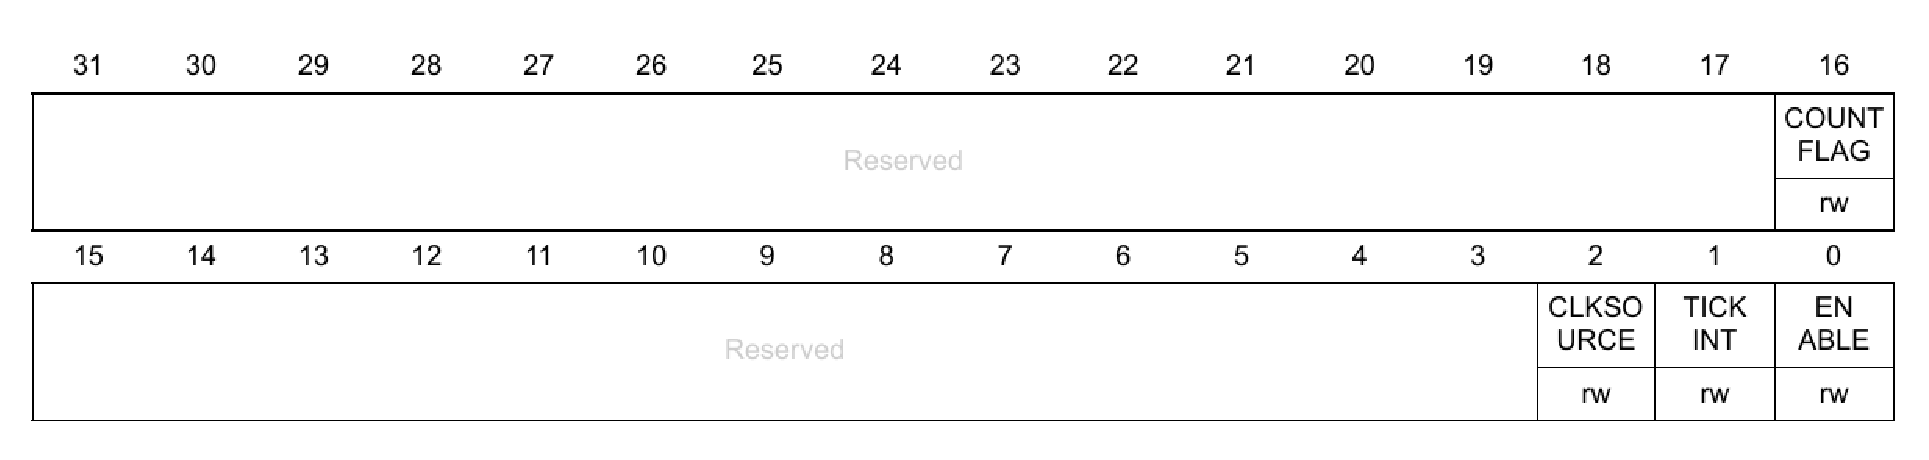
\includegraphics[width=\columnwidth]{./stm32/timers/figs/systick_ctrl.eps}
\end{center}
\caption{Control Register (CTRL)}
\label{fig:systick_ctrl}
\end{figure}
\item What does the following instruciton do?
\begin{lstlisting}
SysTick->CTRL = 0x00000005;	//8MHz clock
\end{lstlisting}
\solution From Fig. \ref{fig:systick_ctrl}, ENABLE = 1 enables the counter (for delay) and CLKSOURCE = 1 enables the 8 MHz internal RC clock.
\item Obtain a 1 MHz clock. 
\\
\solution CLKSOURCE = 1 results in the $\frac{\text{Processor Clock}}{8} = 1$ MHz clock.
\begin{lstlisting}
SysTick->CTRL = 0x00000001;	//1MHz clock
\end{lstlisting}
\item Obtain a delay of 1 second using the 1 MHz clock.
\subsection{TIMER-1}
\item Make the connections according to Table \ref{table:systick_pins}.  Execute the following program
\begin{lstlisting}
cd /timers/timer1_blink.c
\end{lstlisting}
\label{prob:APB2_TIM1}
\item Enable Timer1 through RCC.
\\
\solution 
\begin{lstlisting}
RCC->APB2ENR |= RCC_APB2ENR_TIM1EN;  
\end{lstlisting}
\item Select the HSI clock of 8 MHz as TIM1 clock.
\\
\solution See Fig.  \ref{fig:smcr} for register. SMS=000 implies that the TIM1 will be controlled by the internal clock.
\begin{lstlisting}
TIM1->SMCR  = 0;
\end{lstlisting}
\begin{figure}[!ht]
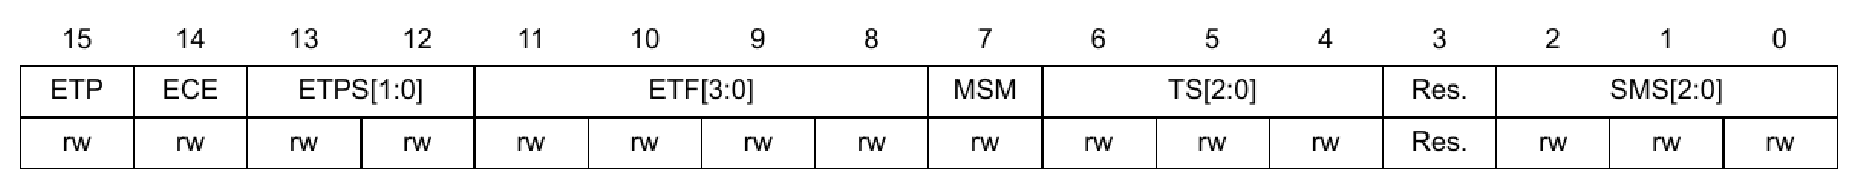
\includegraphics[width=\columnwidth]{./stm32/timers/figs/smcr.eps}
\caption{Slave Mode Control Register (SMCR)}
\label{fig:smcr}
\end{figure}
\item What does the following instruction do?
\begin{lstlisting}
TIM1->CR1 	= 0x0001;
\end{lstlisting}
\solution Fig. \ref{fig:cr1} shows the control register 1 (CR1). CEN=1 enables the counter.
\begin{figure}[!ht]
\begin{center}
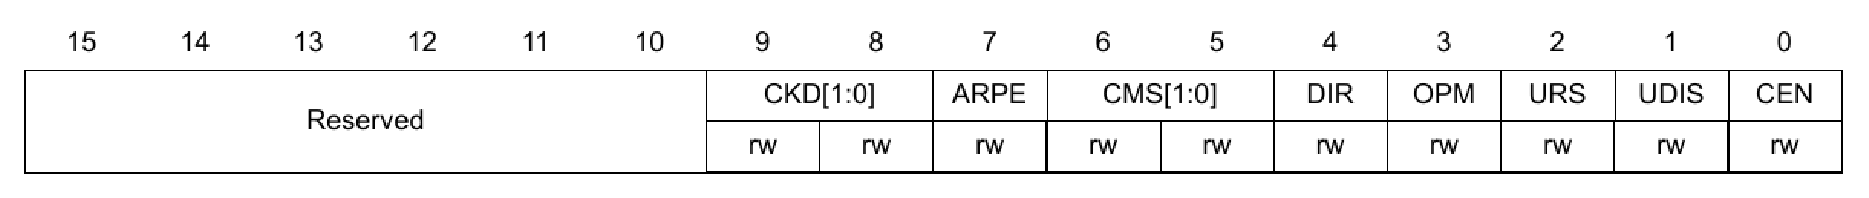
\includegraphics[width=\columnwidth]{./stm32/timers/figs/cr1.eps}
\end{center}
\caption{Control Register 1 (CR1)}
\label{fig:cr1}
\end{figure}
\item Make TIM1 clock = 2 KHz.
\\
\solution Through the following command,
\begin{lstlisting}
TIM1->PSC	= 3999;
\end{lstlisting}
\begin{equation}
TIM1\_CLK = \frac{HSI\_CLK}{TIM1->PSC + 1} = \frac{8000000}{4000}
\end{equation}
Fig. \ref{fig:psc} shows the TIM1$->$PSC (prescalar) register.
\begin{figure}[!ht]
\begin{center}
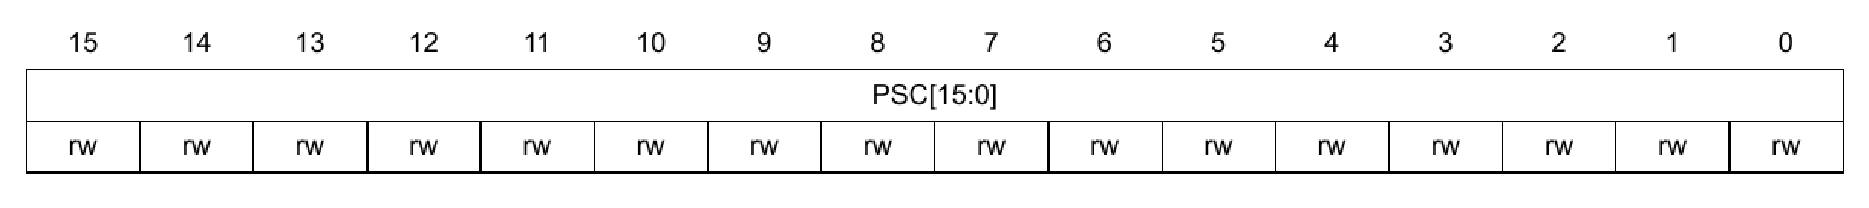
\includegraphics[width=\columnwidth]{./stm32/timers/figs/psc.eps}
\end{center}
\caption{Prescalar (PSC)}
\label{fig:psc}
\end{figure}
\item What is the maximum value that can be stored in TIM1$->$PSC?
\item Make TIM1 count 1000 cycles of the 2 KHz TIM1 clock.
\\
\solution 
\begin{lstlisting}
TIM1->ARR 	= 999;	
\end{lstlisting}
\item Like the PSC, the ARR (auto reload register) is also of length 16 bits and used for factoring the clock.
\item What do the following instructions do?
\begin{lstlisting}
if(TIM1->SR & 0x0001)//check if ARR count complete
{
	TIM1->SR &= ~0x0001;//clear status register SR
	GPIOA->ODR ^= (1 << 1);//blink LED through PA1
}
\end{lstlisting}
\solution Once the TIM1 counter counts from 0 to TIM1$->$ARR=999, it resets and starts counting again to 999.  At the time of
reset, the LSB of TIM1$->$SR = 1.  The \textbf{if} command checks this and when this condition is satisfied, TIM1$->$SR is cleared
and PA1 is toggled.  This process keeps repeating. This results in a PA1  output of 1 and 0 with frequency
\begin{multline}
\frac{HSI\_CLK}{\brak{TIM1->PSC + 1}\brak{TIM1->ARR + 1}} 
\\
= \frac{8000000}{4000\times 1000} = 2 \text{ Hz}
\end{multline}
\item How would you use the repetition counter (RCR) to do the above?
\\
\solution The following instructions
\begin{lstlisting}
	TIM1->SMCR  = 0;	//Internal clock, 8MHz	
	TIM1->PSC	= 999;	//Prescalar, dividing clock by 1000
	TIM1->CR1 	= 0x0001;	//enable Timer1
	TIM1->ARR 	= 999;	//Load Count
	TIM1->RCR 	= 3;	//Load Repetition Count	
\end{lstlisting}
lead to
{\footnotesize
\begin{multline}
\frac{HSI\_CLK}{\brak{TIM1->PSC + 1}\brak{TIM1->ARR + 1}\brak{TIM1->RCR + 1}} 
\\
= \frac{8000000}{4000\times 1000} = 2 \text{ Hz}
\end{multline}
}
TIM1$->$RCR keeps track of the number of times the counter has overflowed. Fig. \ref{fig:rcr} shows the repetition counter register.
\begin{figure}[!h]
\begin{center}
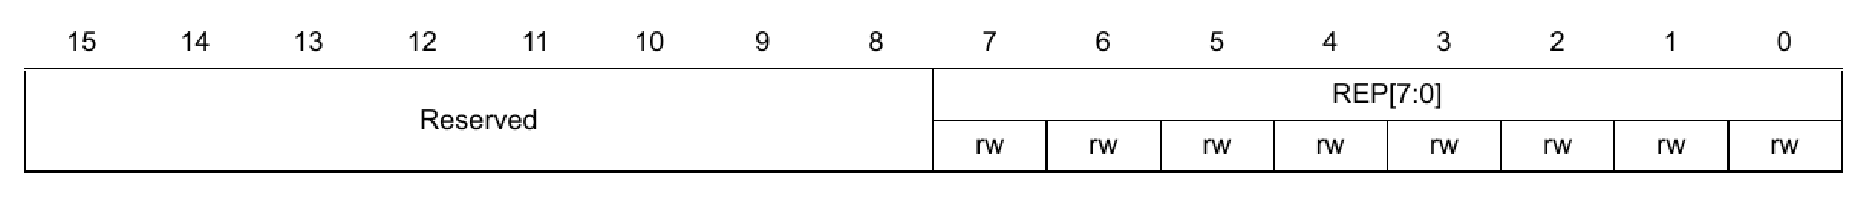
\includegraphics[width=\columnwidth]{./stm32/timers/figs/rcr.eps}
\end{center}
\caption{Repition Counter (RCR)}
\label{fig:rcr}
\end{figure}
\item What is the maximum value of TIM1$->$RCR?
\item What is the function of TIM1$->$SR?
\\
\solution The status register (SR) is shown in Fig. \ref{fig:sr}. The UIF flag is 1 if the RCR overflows.
\begin{figure}[!h]
\begin{center}
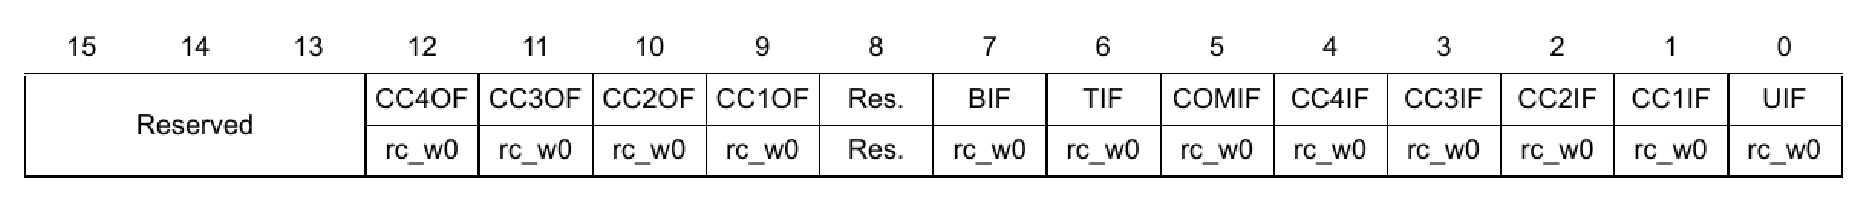
\includegraphics[width=\columnwidth]{./stm32/timers/figs/sr.eps}
\end{center}
\caption{Staus Register (SR)}
\label{fig:sr}
\end{figure}

\subsection{TIMER-2}
\item Blink an LED with TIM2.
\\
\solution 
\begin{lstlisting}
cd timers/timer2_blink.c
\end{lstlisting}
\item In the above code, 
\begin{lstlisting}
RCC->APB1ENR |= RCC_APB1ENR_TIM2EN;
\end{lstlisting}
is used for enabling TIM2. Note that for TIM1, APB2 was used instead of APB1 in Problem \ref{prob:APB2_TIM1}.  Explain.
\\
\solution Advanced Peripheral Bus 1 (APB1) and Advanced Peripheral Bus 2 (APB2) are connected to the Direct Memory Access (DMA) module, SRAM, peripherals like GPIOs, ADC, timers, etc. and Cortex core. APB1 has a maximum operating frequency of 36MHz while the maximum operating frequency of APB2  is 72MHz. That is why GPIOs are connected to APB2 bus instead of APB1 or any other bus and STM32 GPIOs can achieve 50MHz switching speed. APB1 bus mostly serves communication and timer modules of the STM32. 
\item Mention any major difference between TIM1 and TIM2.
\\
\solution TIM1 is an advanced timer while TIM2 is a general purpose timer.  One major difference between the two is that TIM2 does not have RCR.
\subsection{Master-Slave Configuration}
\subsubsection{Blink}
\item Execute the following program.
\begin{lstlisting}
cd timers/master1_slave2_blink.c
\end{lstlisting}
\item List the instructions for setting up TIM1 as master and TIM2 as slave. TIM1 should be a prescalar for TIM2.
\\
\solution The MMS bits can be seen in the CR2 register is shown in Fig. \ref{fig:cr2}. The TS and SMS bits are visible in the SMCR register
in Fig. \ref{fig:smcr}. 
\begin{lstlisting}
TIM1->CR2	= 0x0020;//MMS = 010
TIM2->SMCR	= 0x0007;//TS = 000, SMS = 111	
\end{lstlisting}
%
\begin{figure}[!h]
\begin{center}
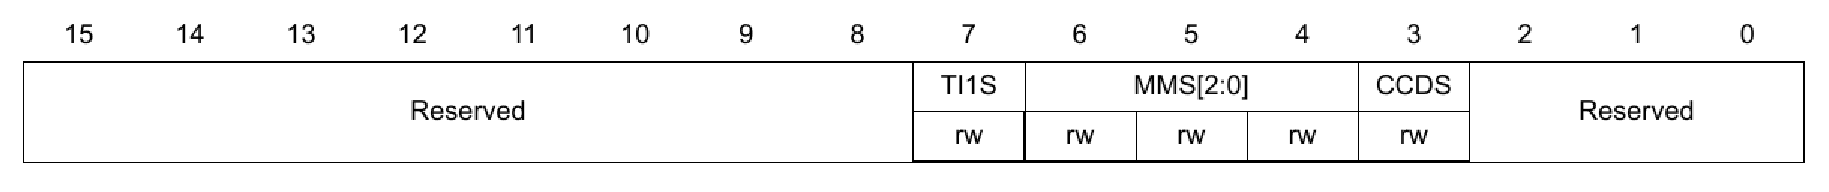
\includegraphics[width=\columnwidth]{./stm32/timers/figs/cr2.eps}
\end{center}
\caption{Control Register 2 (CR2)}
\label{fig:cr2}
\end{figure}
%
\subsubsection{Decade Counter}
\item Execute the following program.
\begin{lstlisting}
cd timers/decade_counter.c
\end{lstlisting}
%
\item If TIM2$->$ARR = 9, TIM2$->$CNT = ?
\\
\solution TIM2$->$CNT = 0, 1, \dots, 9, 0,\dots, 9,\dots The counting rate depends on the PCR, ARR, RCR registers of TIM1 and the PCR
and ARR registers of TIM2.
\end{enumerate}
%\section{Hardware}
%
%%\subsection{Seven Segment Display}
%%The breadboard can be divided into 5 segments.  In each of the green segements, the pins are internally connected so as to have the same voltage.  Similarly, in the central segments, the pins in each column  are internally connected in the same fashion as the blue columns. 
%
%%\begin{problem}
%%	Plug the display to the breadboard in Fig. \ref{fig:breadboard}
%%\end{problem}
%%\begin{figure}[!h]
%%\begin{center}
%%\includegraphics[width=\columnwidth]{./figs/breadboard}
%%\end{center}
%%\caption{}
%%\label{fig:breadboard}
%%\end{figure}
%
%%The seven segment display in Fig. \ref{fig:sevenseg} has eight pins, $a, b, c, d, e, f, g$ and $dot$ that take an active LOW input, i.e.  the LED will glow only if the input is connected to ground.  Each of these pins is connected to an LED segment.  The $dot$ pin is  reserved for the $\cdot$ LED.  
%
%%
%%\begin{center}
%	%\includegraphics[scale=1]{sevenseg}
%%\end{center}
%
%%\begin{problem}
%%	Connect one end of the 1K resistor to the COM pin of the display and the other end to an extreme pin of the breadboard.	
%%\end{problem}
%%%
%%%
%%%
%%\begin{figure}[!h]
%%\begin{center}
%%\resizebox {0.5\columnwidth} {!} {
%%\input{./figs/sevenseg.tex}
%%}
%%\end{center}
%%\caption{}
%%\label{fig:sevenseg}
%%\end{figure}
%
%The STM32F103C8T6 micro-controller in Fig. \ref{fig:stm_blue}
%has two ground pins, few analog input pins and few digital pins that can be used for both input as well as output. It has one Vcc (3.3V) pin that can generate 3.3$V$.  In the following exercises, only the GND, 3.3$V$ and digital pins will be used.
%%
%%
%\begin{problem}
%Make the pin connections in Table \ref{table:stm_ssd} using Figs. \ref{fig:sevenseg} and \ref{fig:stm_blue}.
%	\end{problem}	
%%
%\begin{figure}[!h]
%\begin{center}
%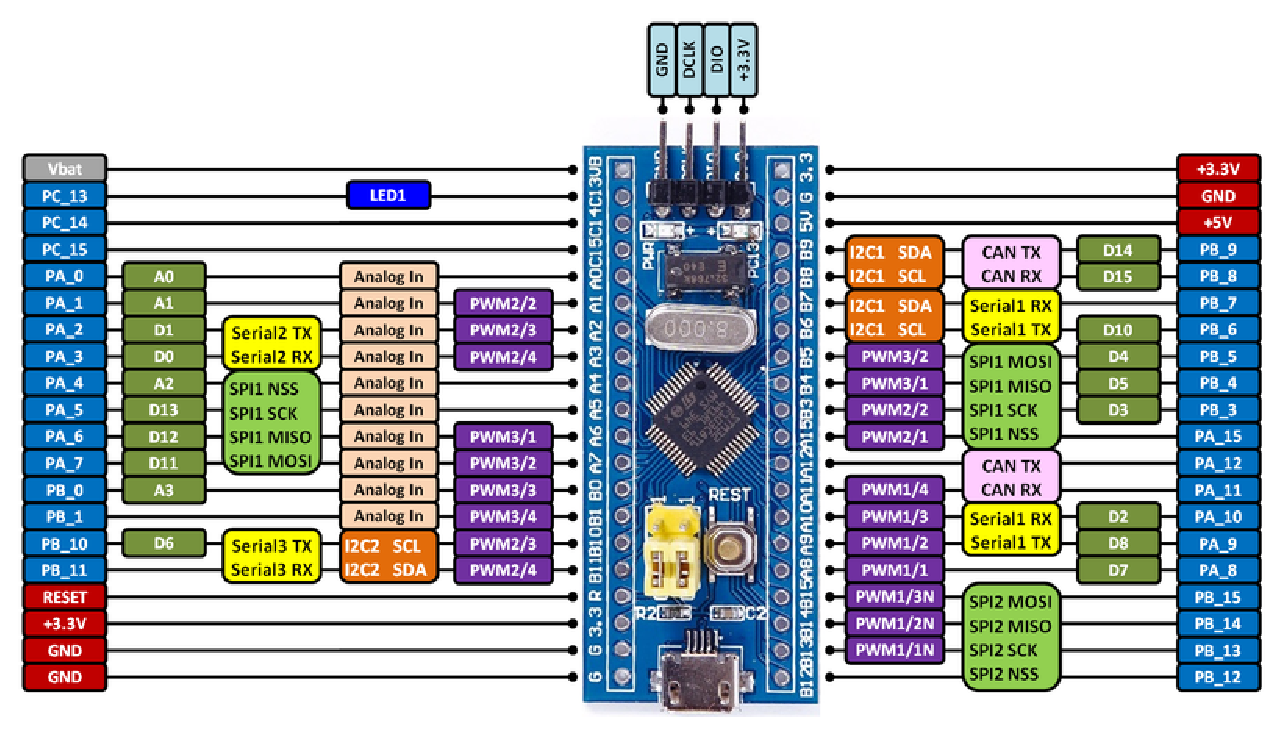
\includegraphics[width=\columnwidth]{./figs/stm_blue.eps}
%\end{center}
%\caption{}
%\label{fig:stm_blue}
%\end{figure}
%%
%\begin{table}
%\small
%\input{./figs/stm_ssd}
%\caption{}
%\label{table:stm_ssd}
%\end{table}
%
%
%\section{Software}
%%
%\begin{problem}
%Execute 
%\begin{lstlisting}
%https://github.com/gadepall/STM32F103C8T6/blob/master/examples/sevenseg_example.c
%\end{lstlisting}
%\end{problem}
%%\begin{problem}
%%	Connect the STM32 to the Raspberry Pi according to the \href{https://github.com/gadepall/EE4013/blob/master/setup/rpi/gvv_stm32_setup.pdf}{\url{instructions }} in
%%\begin{lstlisting}
%%https://github.com/gadepall/EE4013/blob/master/setup/rpi/gvv_stm32_setup.pdf
%%\end{lstlisting}	
%%\end{problem}
%%\section{Display Control with STM32}
%%
%%\begin{problem}
%%Follow the \href{https://github.com/gadepall/EE4013/blob/master/setup/tinker/gvv_stm32_tinker_setup.pdf}{\url{instructions }} in
%%\begin{lstlisting}
%%https://github.com/gadepall/EE4013/blob/master/setup/tinker/gvv_stm32_tinker_setup.pdf
%%\end{lstlisting}
%%to clone the \href{https://github.com/gadepall/EE4013/blob/master/setup/tinker/gvv_stm32_tinker_setup.pdf}{\url{repository }}
%%\begin{lstlisting}[language=bash, frame=single, breaklines]
%%https://github.com/gadepall/STM32F103C8T6
%%\end{lstlisting}
%%\end{problem}
%%
%%Fig. \ref{fig:sevenseg12} explains how to get decimal digits using the seven segment display. 
%%\begin{problem}
%%In the STM32F103C8T6 directory,
%%\begin{lstlisting}
%%cp sevenseg.c main.c
%%\end{lstlisting}
%%Generate the number 0 by executing \textbf{main.c} and flashing to the STM32. 
%%\end{problem}	
%%
%\begin{figure}[!h]
%\begin{center}
%\resizebox {0.8\columnwidth} {!} {
%\input{./figs/sevenseg12.tex}
%}
%\end{center}
%\caption{}
%\label{fig:sevenseg12}
%\end{figure}
%%
%
%\begin{problem}
%Explain the process of generating the number 0 using the following instruction.
%\begin{lstlisting}
%GPIOB->ODR = 0xFC08;
%\end{lstlisting}
%\end{problem}
%\solution ODR is the Output Data Register, which is used to write outputs to the GPIO pins. The 16 bit number 0xFC08 on the RHS represents the pin configuration for the pins of port B of STM32F103C8T6, which are numbered PB15-PB0 in that order.  See Table \ref{table:stm_ssd}, 
%
%\begin{problem}
%	Repeat the above exercise to generate the numbers 1-9 on the display.
%\end{problem}	
%\begin{problem}
%The previous instructions set the bits in the unused ports PB15-PB10 and PB2-PB0. This may be undesirable in some cases. Generate 0 by not disturbing 
%the unused pins.
%\end{problem}
%\solution The following instructions help accomplish this. The first instruction resets PB4-PB9.  The second instruction sets the PB3 pin. The other pins are
%undisturbed.
%\begin{lstlisting}
%GPIOB->BRR = (1<<4)|(1<<5)|(1<<6)|(1<<7)|(1<<8)|(1<<9); // (Led ON)		
%GPIOB->BSRR = (1<<3); // (Led OFF)					
%\end{lstlisting}
%%\section{Manual Display Control}
%%\input{./chapters/chapter1}
%%
%\begin{problem}
%Write a program to take a 4-bit BCD as input from hardware (GND or VDD) and show the next number on the seven segment display.
%\end{problem}
%%
%\solution The following program takes 4 bits as input from pins PB12-PB15 and displays the output on a seven segment display. The next number
%can be displayed by slightly modifying the code.
%\begin{lstlisting}
%https://github.com/gadepall/STM32F103C8T6/blob/master/examples/bin2dec_example.c
%\end{lstlisting}
